\documentclass[landscape]{slides}
\usepackage{url}
\usepackage{amsmath}
\usepackage{graphicx}
\usepackage{color}
\usepackage{epic,ecltree}
\usepackage{eclbip}
\usepackage{multicol}
\usepackage{algorithmic}
\usepackage{algorithm}
\renewcommand{\algorithmicrequire}{\textbf{Input:}}
\renewcommand{\algorithmicensure}{\textbf{Output:}}
\renewcommand{\algorithmiccomment}[1]{// {\em #1}}

\definecolor{darkblue}{rgb}{0,0,0.8}
\definecolor{darkgreen}{rgb}{0,0.8,0}
\definecolor{reddishgreen}{rgb}{0.4,0.6,0}
\definecolor{purple}{rgb}{0.6,0,0.6}
\definecolor{red}{rgb}{1,0,0}

\newcommand{\example}[1]{\textcolor{darkblue}{\rm #1}}
\newcommand{\maths}[1]{\textcolor{purple}{#1}}
\newcommand{\reference}[1]{\vspace{-2mm}\begin{flushright}\textcolor{purple}{\tiny [from #1]}\end{flushright}\vspace{-7mm}}

\begin{document}
\title[Chapter 8: Evaluation]{Chapter 8\\[1cm] Evaluation}
\author[Philipp Koehn]{}
\date{Statistical Machine Translation}

\maketitle

%%%%%%%%%%%%%%%%%%%%%%%%%%%%%%%%%%%%%%%%%%%%%%%%%%%%%%%%%%%%%%%%%%%%%%%%%%%%

\slide{Evaluation}
\vspace{10mm}
\begin{itemize}
\item How good is a given machine translation system?
\item Hard problem, since many different translations acceptable\\
$\rightarrow$ semantic equivalence / similarity
\item Evaluation metrics
\begin{itemize}
\item subjective judgments by human evaluators
\item automatic evaluation metrics
\item task-based evaluation, e.g.:
\begin{itemize}
\item[--] how much post-editing effort?
\item[--] does information come across? 
\end{itemize}
\end{itemize}
\end{itemize}

%%%%%%%%%%%%%%%%%%%%%%%%%%%%%%%%%%%%%%%%%%%%%%%%%%%%%%%%%%%%%%%%%%%%%%%%%%%%

\slide{Ten Translations of a Chinese Sentence}
\vspace{5mm}
\begin{center}\example{
\begin{tabular}{l}

\includegraphics[width=18cm]{chinese-israel-airport-security.png}\\
Israeli officials are responsible for airport security.\\
Israel is in charge of the security at this airport.\\
The security work for this airport is the responsibility of the Israel government.\\
Israeli side was in charge of the security of this airport.\\
Israel is responsible for the airport's security.\\
Israel is responsible for safety work at this airport.\\
Israel presides over the security of the airport.\\
Israel took charge of the airport security.\\
The safety of this airport is taken charge of by Israel.\\
This airport's security is the responsibility of the Israeli security officials.
\end{tabular}
}

(a typical example from the 2001 NIST evaluation set)
\end{center}

%%%%%%%%%%%%%%%%%%%%%%%%%%%%%%%%%%%%%%%%%%%%%%%%%%%%%%%%%%%%%%%%%%%%%%%%%%%%

\slide{Adequacy and Fluency}
\vspace{10mm}
\begin{itemize}
\item Human judgement
\begin{itemize}
\item given: machine translation output
\item given: source and/or reference translation
\item task: assess the quality of the machine translation output
\end{itemize}
\item Metrics
\begin{description}
\item[{\bf Adequacy:}\index{adequacy}] Does the output convey the same meaning as the input sentence?\\ Is part of the message lost, added, or distorted?\vspace{3mm}
\item[{\bf Fluency:}\index{fluency}] Is the output good fluent English?\\ This involves both grammatical correctness and idiomatic word choices. \vspace{3mm}
\end{description}
\end{itemize}

%%%%%%%%%%%%%%%%%%%%%%%%%%%%%%%%%%%%%%%%%%%%%%%%%%%%%%%%%%%%%%%%%%%%%%%%%%%%

\slide{Fluency and Adequacy: Scales}
\vspace{40mm}
\begin{center}
\begin{tabular}{|c|c|p{2cm}|c|c|} \cline{0-1} \cline{4-5}
\multicolumn{2}{|c|}{\bf Adequacy} & & \multicolumn{2}{|c|}{\bf Fluency} \\ \cline{0-1} \cline{4-5}
5 & all meaning &    & 5 & flawless English \\ \cline{0-1} \cline{4-5}
4 & most meaning &   & 4 & good  English \\ \cline{0-1} \cline{4-5}
3 & much meaning &   & 3 & non-native English \\ \cline{0-1} \cline{4-5}
2 & little meaning & & 2 & disfluent English \\ \cline{0-1} \cline{4-5}
1 & none &           & 1 & incomprehensible \\ \cline{0-1} \cline{4-5}
\end{tabular}
\end{center}


%%%%%%%%%%%%%%%%%%%%%%%%%%%%%%%%%%%%%%%%%%%%%%%%%%%%%%%%%%%%%%%%%%%%%%%%%%%%

\slide{Annotation Tool}
\begin{center}
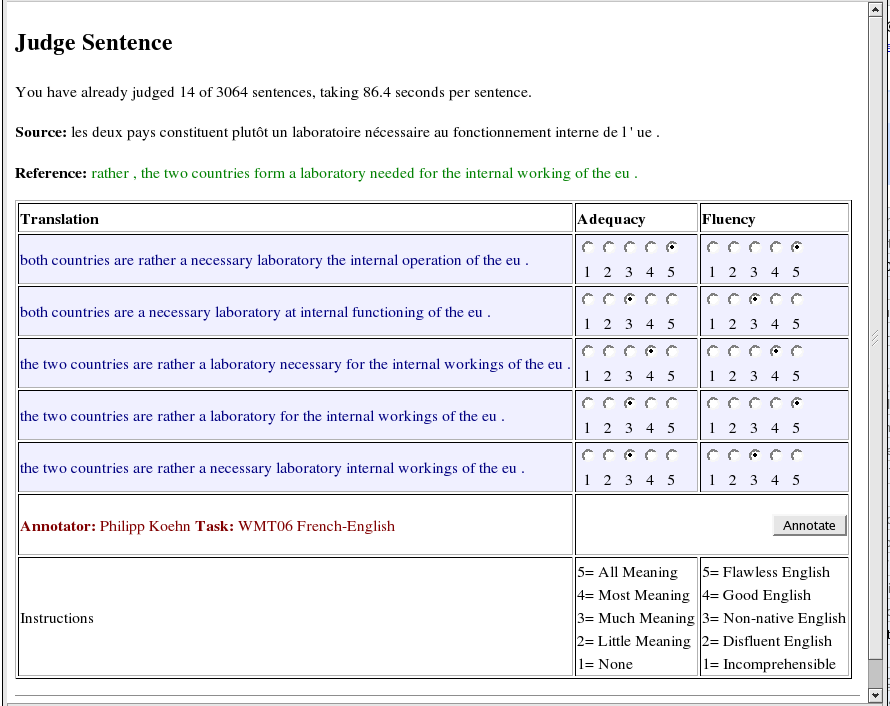
\includegraphics[width=17.2cm]{evaluation-tool.png}
\end{center}

%%%%%%%%%%%%%%%%%%%%%%%%%%%%%%%%%%%%%%%%%%%%%%%%%%%%%%%%%%%%%%%%%%%%%%%%%%%%

\slide{Evaluators Disagree}
\vspace{10mm}
\begin{itemize}
\item Histogram of adequacy judgments by different human evaluators
\end{itemize}
\begin{center}
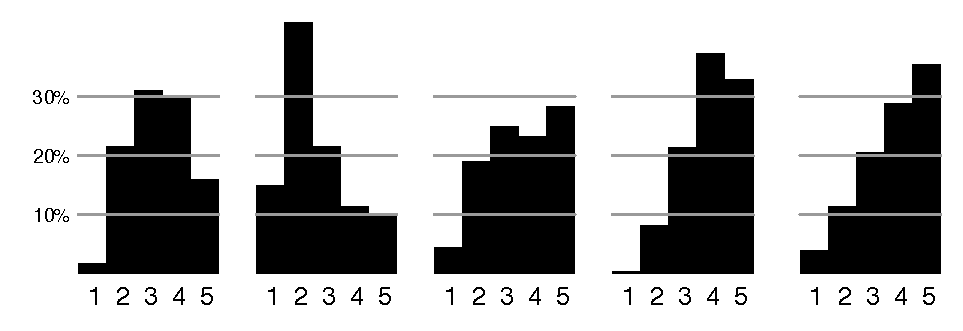
\includegraphics[scale=1.4]{adequacy-histograms.pdf}\\
(from WMT 2006 evaluation)
\end{center}

%%%%%%%%%%%%%%%%%%%%%%%%%%%%%%%%%%%%%%%%%%%%%%%%%%%%%%%%%%%%%%%%%%%%%%%%%%%%

\slide{Measuring Agreement between Evaluators}
\vspace{5mm}
\begin{itemize}
\item Kappa coefficient
\maths{\begin{equation*}
K = \frac{p(A) - p(E)}{1 - p(E)}
\end{equation*}}
\begin{itemize}
\item \maths{$p(A)$}: proportion of times that the evaluators agree
\item \maths{$p(E)$}: proportion of time that they would agree by chance\\
(5-point scale $\rightarrow$ \maths{$p(E)=\frac{1}{5}$})
\end{itemize}
\item Example: Inter-evaluator agreement in WMT 2007 evaluation campaign
\begin{center}
\begin{tabular}{lccc}
Evaluation type & $P(A)$ & $P(E)$ & $K$ \\
\hline
Fluency & .400 & .2 & .250\\
Adequacy & .380 &  .2 & .226\\
\hline
\end{tabular}
\end{center}
\end{itemize}

%%%%%%%%%%%%%%%%%%%%%%%%%%%%%%%%%%%%%%%%%%%%%%%%%%%%%%%%%%%%%%%%%%%%%%%%%%%%

\slide{Ranking Translations}
\vspace{20mm}
\begin{itemize}
\item Task for evaluator: Is translation X better than translation Y?\\
(choices: better, worse, equal)
\vspace{5mm}
\item Evaluators are more consistent:

\begin{center}
\begin{tabular}{lccc}
Evaluation type & $P(A)$ & $P(E)$ & $K$ \\
\hline
Fluency & .400 & .2 & .250\\
Adequacy & .380 &  .2 & .226\\
Sentence ranking & .582 & .333 & .373\\
\hline
\end{tabular}
\end{center}

\end{itemize}

%%%%%%%%%%%%%%%%%%%%%%%%%%%%%%%%%%%%%%%%%%%%%%%%%%%%%%%%%%%%%%%%%%%%%%%%%%%%

\slide{Goals for Evaluation Metrics}
\vspace{25mm}
\begin{description}
\item[Low cost:] reduce time and money spent on carrying out evaluation
\item[Tunable:] automatically optimize system performance towards metric
\item[Meaningful:] score should give intuitive interpretation of translation quality
\item[Consistent:] repeated use of metric should give same results
\item[Correct:] metric must rank better systems higher
\end{description}

%%%%%%%%%%%%%%%%%%%%%%%%%%%%%%%%%%%%%%%%%%%%%%%%%%%%%%%%%%%%%%%%%%%%%%%%%%%%

\slide{Other Evaluation Criteria}
\vspace{27mm}
When deploying systems, considerations go beyond quality of translations
\vspace{5mm}
\begin{description}
\item[Speed:] we prefer faster machine translation systems
\item[Size:] fits into memory of available machines (e.g., handheld devices)
\item[Integration:] can be integrated into existing workflow
\item[Customization:] can be adapted to user's needs 
\end{description}

%%%%%%%%%%%%%%%%%%%%%%%%%%%%%%%%%%%%%%%%%%%%%%%%%%%%%%%%%%%%%%%%%%%%%%%%%%%%

\slide{Automatic Evaluation Metrics}
\vspace{20mm}
\begin{itemize}
\item Goal: computer program that computes the quality of translations
\item Advantages: low cost, tunable, consistent
\vspace{5mm}
\item Basic strategy
\begin{itemize}
\item given: machine translation output
\item given: human reference translation
\item task: compute similarity between them
\end{itemize}
\end{itemize}

%%%%%%%%%%%%%%%%%%%%%%%%%%%%%%%%%%%%%%%%%%%%%%%%%%%%%%%%%%%%%%%%%%%%%%%%%%%%

\slide{Precision and Recall of Words}
\vspace{5mm}
\begin{center}
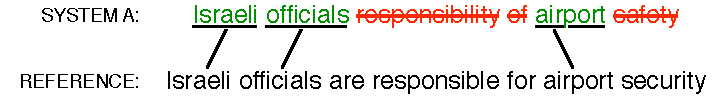
\includegraphics[scale=2]{word-error-rate1.pdf}
\end{center}
\begin{itemize}
\item Precision\vspace{-5mm}
\maths{\begin{equation*}
\frac{\text{\em correct}}{\text{\em output-length}} = \frac{3}{6} = 50\%
\end{equation*}}
\item Recall\vspace{-5mm}
\maths{\begin{equation*}
\frac{\text{\em correct}}{\text{\em reference-length}} = \frac{3}{7} = 43\%
\end{equation*}}
\item F-measure\vspace{-5mm}
\maths{\begin{equation*}
\frac{\text{\em precision} \times \text{\em recall}}{(\text{\em precision} + \text{\em recall})/2} = \frac{.5 \times .43}{(.5+.43)/2} = 46\%
\end{equation*}}
\end{itemize}

%%%%%%%%%%%%%%%%%%%%%%%%%%%%%%%%%%%%%%%%%%%%%%%%%%%%%%%%%%%%%%%%%%%%%%%%%%%%

\slide{Precision and Recall}
\vspace{5mm}
\begin{center}
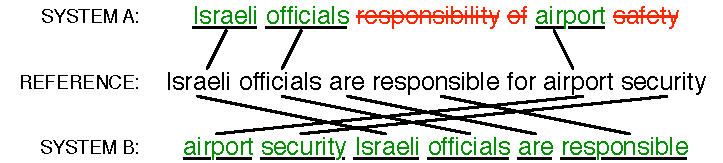
\includegraphics[scale=2]{word-error-rate2.pdf}

\vspace{10mm}
\begin{tabular}{c|c|c}
\bf Metric & \bf System A & \bf System B \\ \hline 
precision & 50\% & 100\% \\ \hline
recall & 43\% & 100\% \\ \hline
f-measure & 46\% & 100\% \\ \hline
\end{tabular}
\vspace{10mm}

flaw: no penalty for reordering
\end{center}


%%%%%%%%%%%%%%%%%%%%%%%%%%%%%%%%%%%%%%%%%%%%%%%%%%%%%%%%%%%%%%%%%%%%%%%%%%%%

\slide{Word Error Rate}
\vspace{10mm}
\begin{itemize}
\item Minimum number of editing steps to transform output to reference
\begin{description}
\item[match:] words match, no cost
\item[substitution:] replace one word with another
\item[insertion:] add word
\item[deletion:] drop word
\end{description}
\item Levenshtein distance
\maths{\begin{equation*}
\text{{\sc wer}} = \frac{\text{\em substitutions} + \text{\em insertions} + \text{\em deletions}}{\text{\em reference-length}}
\end{equation*}}
\end{itemize}

%%%%%%%%%%%%%%%%%%%%%%%%%%%%%%%%%%%%%%%%%%%%%%%%%%%%%%%%%%%%%%%%%%%%%%%%%%%%

\slide{Example}
\vspace{-5mm}
\begin{center}
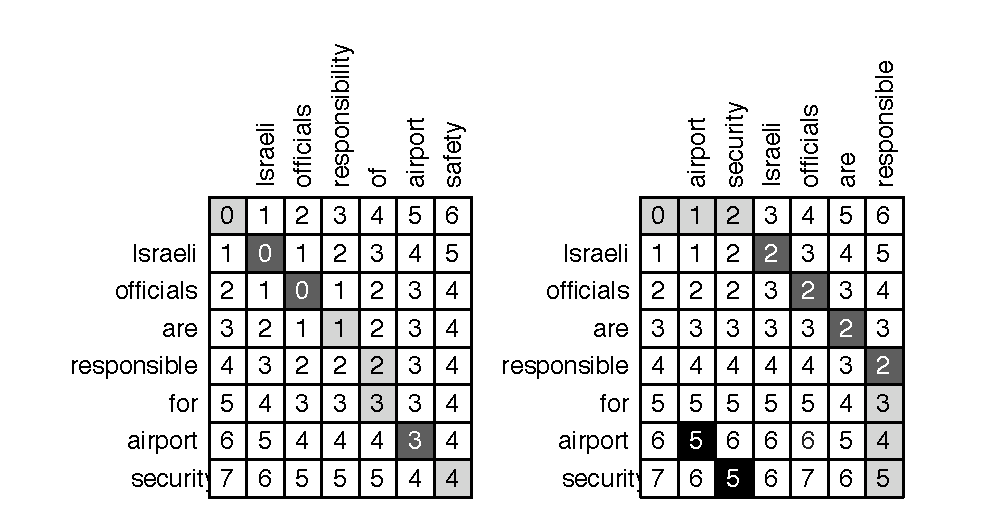
\includegraphics[scale=1.23]{levenshtein.pdf}

\vspace{5mm}
\begin{tabular}{c|c|c}
\bf Metric & \bf System A & \bf System B \\ \hline
word error rate ({\sc wer}) & 57\% & 71\% \\ \hline
\end{tabular}
\end{center}

%%%%%%%%%%%%%%%%%%%%%%%%%%%%%%%%%%%%%%%%%%%%%%%%%%%%%%%%%%%%%%%%%%%%%%%%%%%%

\slide{BLEU}
\vspace{10mm}
\begin{itemize}
\item N-gram overlap between machine translation output and reference translation
\item Compute precision for n-grams of size 1 to 4
\item Add brevity penalty (for too short translations)
\maths{\begin{equation*}
\text{\sc bleu} = \min \left( 1,\frac{\text{\em output-length}}{\text{\em reference-length}} \right) \; \big( \prod_{i=1}^4 \text{\em precision}_i \big)^\frac{1}{4}
\end{equation*}}
\item Typically computed over the entire corpus, not single sentences
\end{itemize}

%%%%%%%%%%%%%%%%%%%%%%%%%%%%%%%%%%%%%%%%%%%%%%%%%%%%%%%%%%%%%%%%%%%%%%%%%%%%

\slide{Example}
\begin{center}
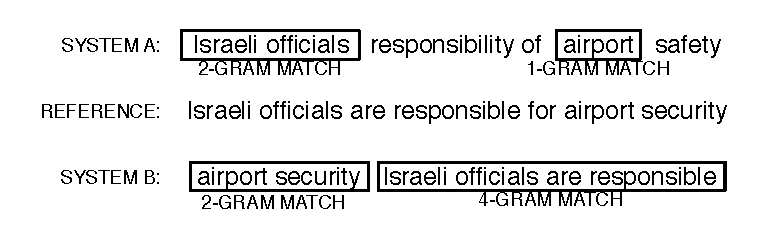
\includegraphics[scale=1.5]{bleu-example.pdf}

\begin{tabular}{c|c|c}
{\bf Metric} & \bf System A & \bf System B \\ \hline
precision (1gram) & 3/6 & 6/6 \\ \hline
precision (2gram) & 1/5 & 4/5 \\ \hline
precision (3gram) & 0/4 & 2/4 \\ \hline
precision (4gram) & 0/3 & 1/3  \\ \hline
brevity penalty   & 6/7 & 6/7  \\ \hline 
{\sc bleu} &  0\% & 52\%  \\ \hline
\end{tabular}
\end{center}


%%%%%%%%%%%%%%%%%%%%%%%%%%%%%%%%%%%%%%%%%%%%%%%%%%%%%%%%%%%%%%%%%%%%%%%%%%%%

\slide{Multiple Reference Translations}
\vspace{10mm}
\begin{itemize}
\item To account for variability, use multiple reference translations
\begin{itemize}
\item n-grams may match in any of the references
\item closest reference length used
\end{itemize}
\item Example\vspace{5mm}
\end{itemize}
\begin{center}
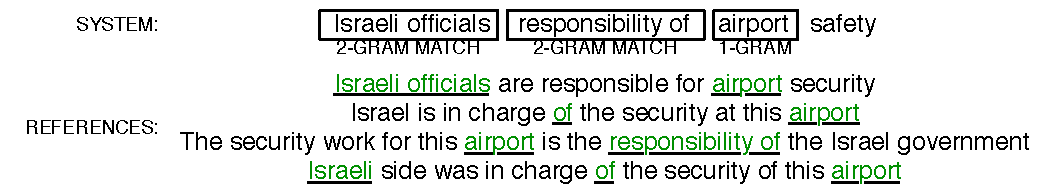
\includegraphics[scale=1.4]{multi-bleu-example-color.pdf}
\end{center}

%%%%%%%%%%%%%%%%%%%%%%%%%%%%%%%%%%%%%%%%%%%%%%%%%%%%%%%%%%%%%%%%%%%%%%%%%%%%

\slide{METEOR: Flexible Matching}
\vspace{10mm}
\begin{itemize}
\item Partial credit for matching stems
\begin{center}
\begin{tabular}{rl}
{\sc system} & \example{\textcolor{red}{Jim} \textcolor{reddishgreen}{went} \textcolor{darkgreen}{home}}\\
{\sc reference} & \example{Joe goes home}\\
\end{tabular}
\end{center}
\item Partial credit for matching synonyms
\begin{center}
\begin{tabular}{rl}
{\sc system} & \example{\textcolor{red}{Jim} \textcolor{reddishgreen}{walks} \textcolor{darkgreen}{home}}\\
{\sc reference} & \example{Joe goes home}\\
\end{tabular}
\end{center}
\item Use of paraphrases
\end{itemize}

%%%%%%%%%%%%%%%%%%%%%%%%%%%%%%%%%%%%%%%%%%%%%%%%%%%%%%%%%%%%%%%%%%%%%%%%%%%%

\slide{Critique of Automatic Metrics}
\vspace{10mm}
\begin{itemize}
\item Ignore relevance of words\\[3mm]
(names and core concepts more important than determiners and punctuation)
\item Operate on local level\\[3mm]
(do not consider overall grammaticality of the sentence or sentence meaning)
\item Scores are meaningless\\[3mm]
(scores very test-set specific, absolute value not informative)
\item Human translators score low on BLEU\\[3mm]
(possibly because of higher variability, different word choices)
\end{itemize}

%%%%%%%%%%%%%%%%%%%%%%%%%%%%%%%%%%%%%%%%%%%%%%%%%%%%%%%%%%%%%%%%%%%%%%%%%%%%

\slide{Evaluation of Evaluation Metrics}
\vspace{40mm}
\begin{itemize}
\item Automatic metrics are low cost, tunable, consistent
\item But are they correct?
\item[$\rightarrow$] Yes, if they correlate with human judgement
\end{itemize}


%%%%%%%%%%%%%%%%%%%%%%%%%%%%%%%%%%%%%%%%%%%%%%%%%%%%%%%%%%%%%%%%%%%%%%%%%%%%

\slide{Correlation with Human Judgement}
\begin{center}\vspace{-5mm}
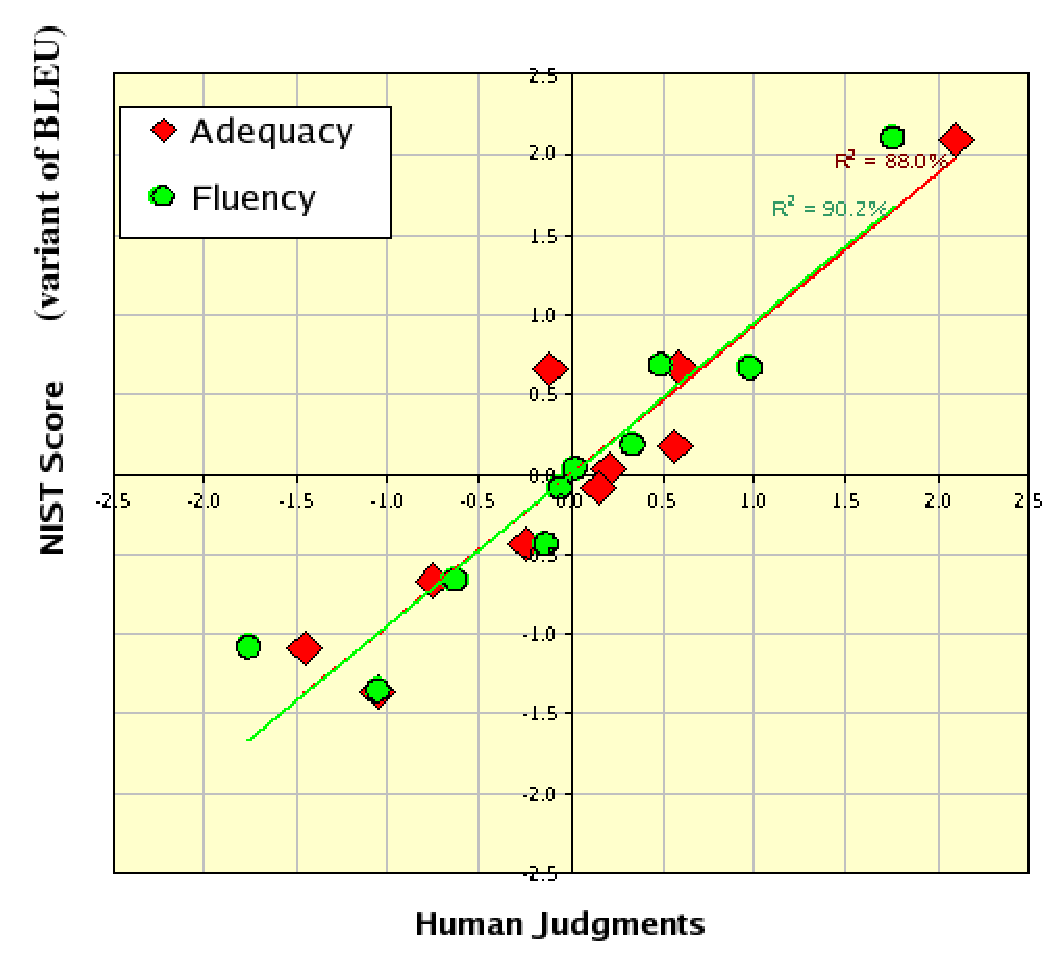
\includegraphics[scale=0.85]{bleu-adequacy-fluency.pdf}
\end{center} 

%%%%%%%%%%%%%%%%%%%%%%%%%%%%%%%%%%%%%%%%%%%%%%%%%%%%%%%%%%%%%%%%%%%%%%%%%%%%

\slide{Pearson's Correlation Coefficient}
\begin{itemize}
\item Two variables: automatic score \maths{$x$}, human judgment \maths{$y$}
\item Multiple systems \maths{$(x_1,y_1)$},  \maths{$(x_2,y_2)$}, ...
\item Pearson's correlation coefficient \maths{$r_{xy}$}:\vspace{-3mm}
\maths{\begin{equation*}
r_{xy} = \frac{\sum_i (x_i-\bar{x}) (y_i-\bar{y})}{(n-1) \; s_x \; s_y}
\end{equation*}}
\vspace{-3mm}
\item Note:\vspace{-20mm}
\maths{\begin{equation*}
\begin{split}
\text{mean} \; \; \bar{x} &= \frac{1}{n} \sum_{i=1}^n x_i\\
\text{variance} \; \; s_x^2 &= \frac{1}{n-1} \sum_{i=1}^n (x_i - \bar{x})^2
\end{split}
\end{equation*}}
\end{itemize}

%%%%%%%%%%%%%%%%%%%%%%%%%%%%%%%%%%%%%%%%%%%%%%%%%%%%%%%%%%%%%%%%%%%%%%%%%%%%

\slide{Metric Research}
\vspace{20mm}
\begin{itemize} \itemsep 10mm
\item Active development of new metrics
\begin{itemize}
\item syntactic similarity
\item semantic equivalence or entailment
\item metrics targeted at reordering
\item trainable metrics
\item etc.
\end{itemize}
\item Evaluation campaigns that rank metrics\\
(using Pearson's correlation coefficient)
\end{itemize}

%%%%%%%%%%%%%%%%%%%%%%%%%%%%%%%%%%%%%%%%%%%%%%%%%%%%%%%%%%%%%%%%%%%%%%%%%%%%

\slide{Evidence of Shortcomings of Automatic Metrics}
\begin{center}
Post-edited output vs. statistical systems (NIST 2005)\\[5mm]
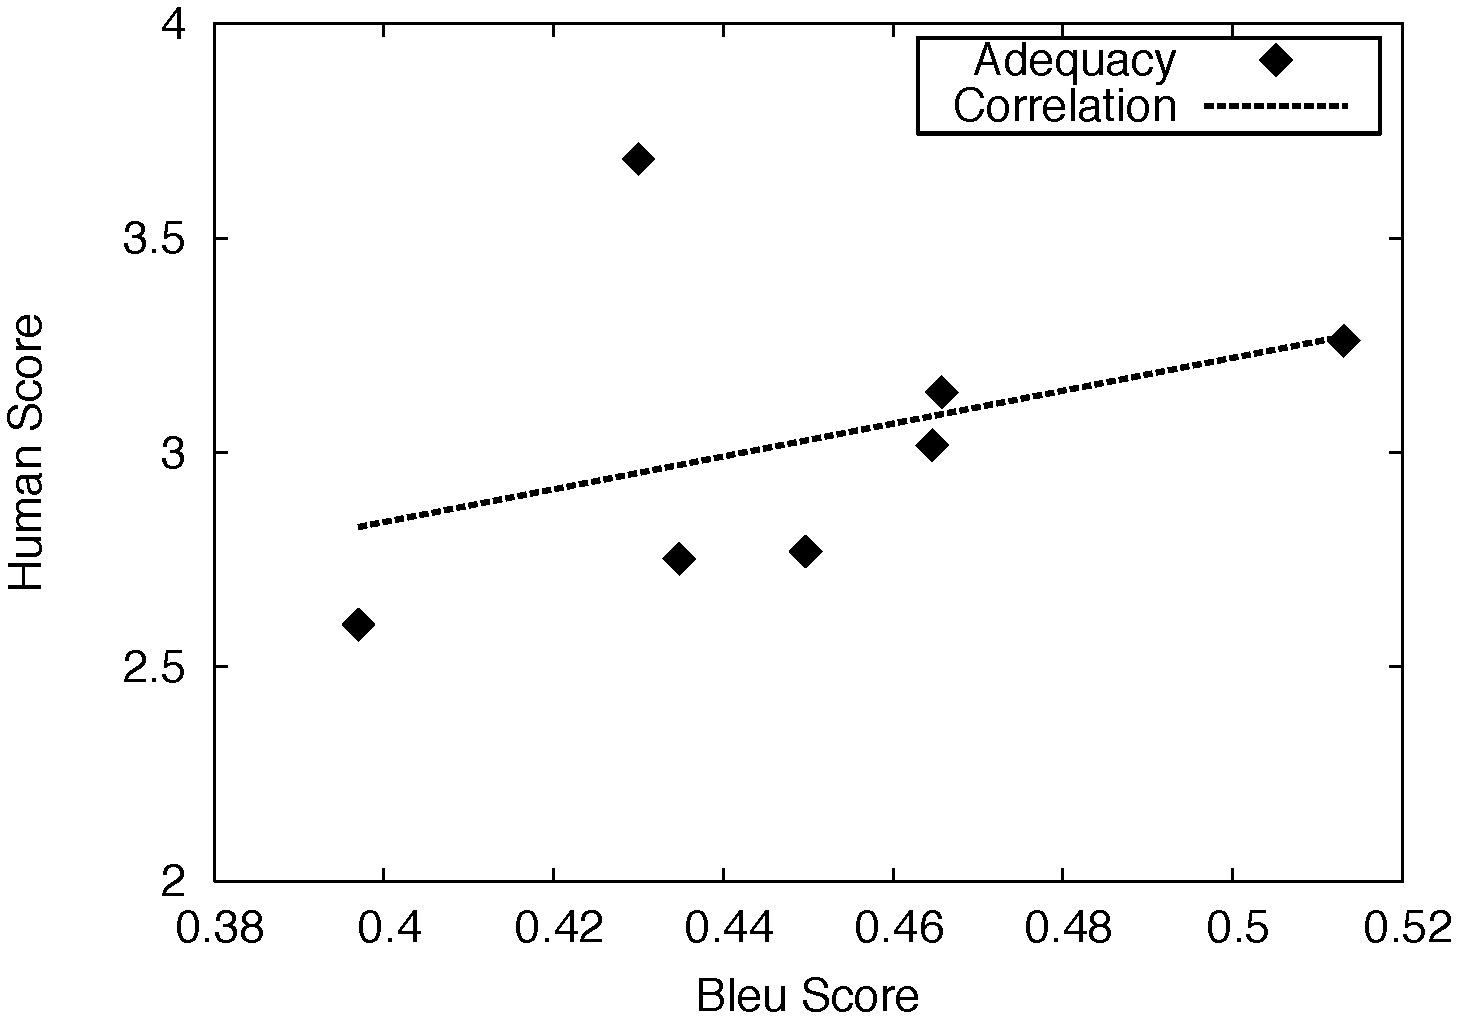
\includegraphics[scale=0.7]{correlation_graph_adequacy.pdf}
\end{center}

%%%%%%%%%%%%%%%%%%%%%%%%%%%%%%%%%%%%%%%%%%%%%%%%%%%%%%%%%%%%%%%%%%%%%%%%%%%%

\slide{Evidence of Shortcomings of Automatic Metrics}
\begin{center}
Rule-based vs. statistical systems\\[5mm]
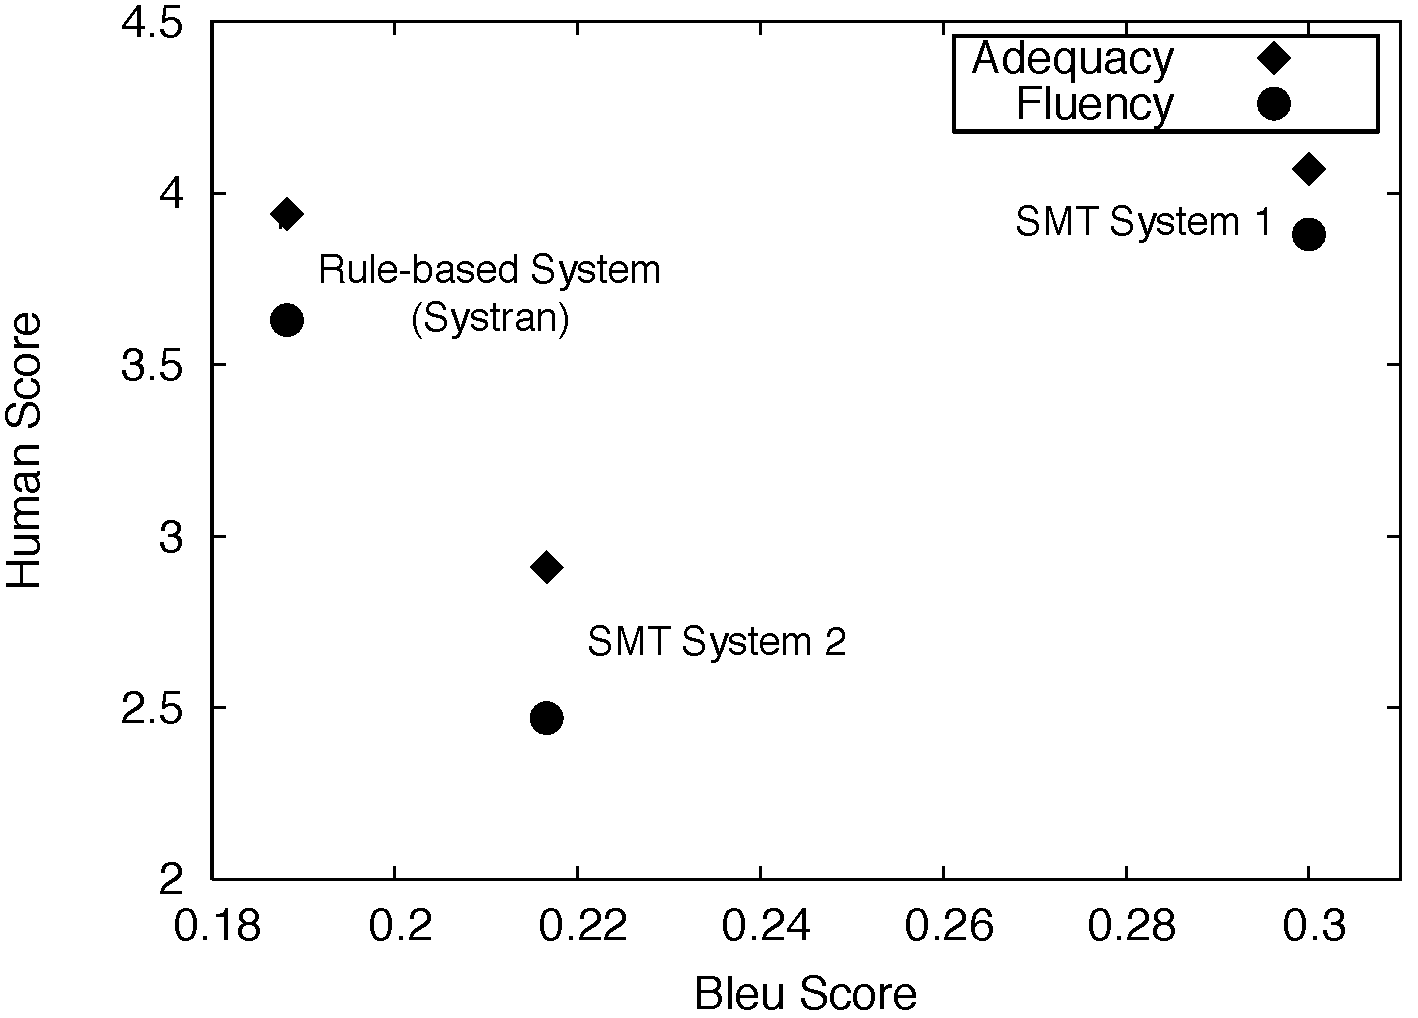
\includegraphics[scale=0.7]{systrans_graph.pdf}
\end{center}

%%%%%%%%%%%%%%%%%%%%%%%%%%%%%%%%%%%%%%%%%%%%%%%%%%%%%%%%%%%%%%%%%%%%%%%%%%%%

\slide{Automatic Metrics: Conclusions}
\vspace{35mm}
\begin{itemize} \itemsep 10mm
\item Automatic metrics essential tool for system development
\item Not fully suited to rank systems of different types 
\item Evaluation metrics still open challenge
\end{itemize}


%%%%%%%%%%%%%%%%%%%%%%%%%%%%%%%%%%%%%%%%%%%%%%%%%%%%%%%%%%%%%%%%%%%%%%%%%%%%

\slide{Hypothesis Testing}
\vspace{20mm}
\begin{itemize}
\item Situation
\begin{itemize}
\item system A has score \maths{$x$} on a test set
\item system B has score \maths{$y$} on the same test set
\item \maths{$x > y$}
\end{itemize}
\item Is system A really better than system B?
\item In other words:\\
Is the difference in score {\bf statistically significant}?
\end{itemize}

%%%%%%%%%%%%%%%%%%%%%%%%%%%%%%%%%%%%%%%%%%%%%%%%%%%%%%%%%%%%%%%%%%%%%%%%%%%%

\slide{Core Concepts}
\vspace{10mm}
\begin{itemize}
\item Null hypothesis
\begin{itemize}
\item assumption that there is no real difference
\end{itemize}
\item P-Levels
\begin{itemize}
\item related to probability that there is a true difference
\item p-level \maths{$p<0.01$} = more than \maths{99\%} chance that difference is real
\item typcically used: p-level \maths{$0.05$} or \maths{$0.01$}
\end{itemize}
\item Confidence Intervals
\begin{itemize}
\item given that the measured score is \maths{$x$}
\item what is the true score (on a infinite size test set)?
\item interval \maths{$[x-d,x+d]$} contains true score with, e.g., 95\% probability
\end{itemize}
\end{itemize}

%%%%%%%%%%%%%%%%%%%%%%%%%%%%%%%%%%%%%%%%%%%%%%%%%%%%%%%%%%%%%%%%%%%%%%%%%%%%

\slide{Computing Confidence Intervals}
\vspace{30mm}
\begin{itemize} \itemsep 10mm
\item Example
\begin{itemize}
\item 100 sentence translations evaluated
\item 30 found to be correct
\end{itemize}
\item True translation score?\\[5mm]
(i.e. probability that any randomly chosen sentence is correctly translated)
\end{itemize}

%%%%%%%%%%%%%%%%%%%%%%%%%%%%%%%%%%%%%%%%%%%%%%%%%%%%%%%%%%%%%%%%%%%%%%%%%%%%

\slide{Normal Distribution}
\begin{center}
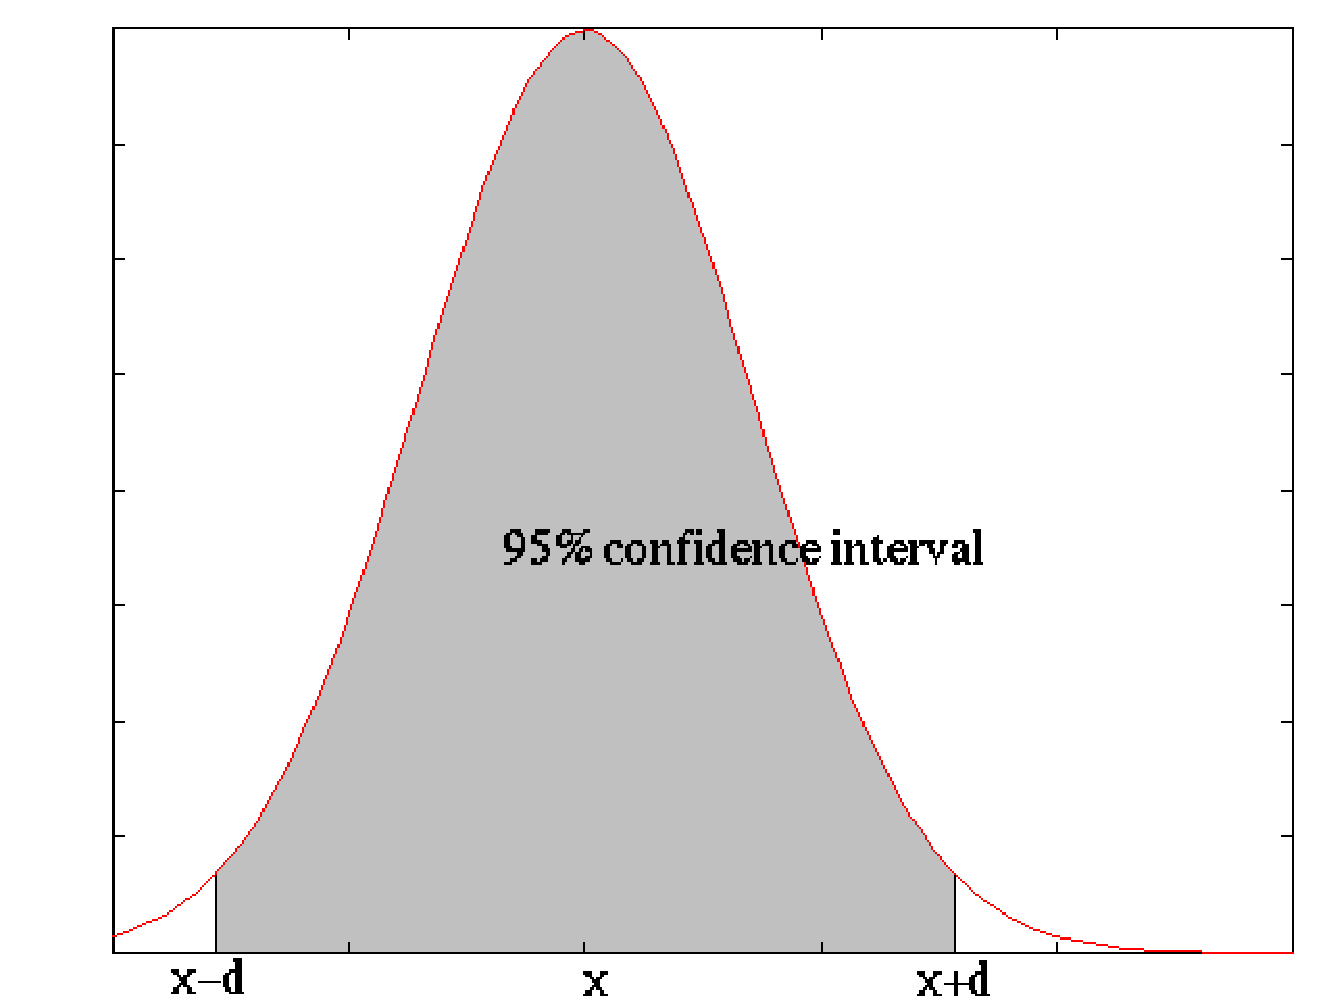
\includegraphics[scale=0.65]{distribution.pdf}\\[5mm]
true score lies in interval \maths{$[\bar{x}-d,\bar{x}+d]$} around sample score \maths{$\bar{x}$}\\
with probability 0.95
\end{center}

%%%%%%%%%%%%%%%%%%%%%%%%%%%%%%%%%%%%%%%%%%%%%%%%%%%%%%%%%%%%%%%%%%%%%%%%%%%%

\slide{Confidence Interval for Normal Distribution}
\vspace{10mm}
\begin{itemize}
\item Compute mean \maths{$\bar{x}$} and variance \maths{$\bar{s^2}$} from data
\maths{\begin{equation*}
\begin{split}
\bar{x} =& \frac{1}{n} \sum_{i=1}^n x_i \\
s^2 =& \frac{1}{n-1} \sum_{i=1}^n (x_i - \bar{x})^2
\end{split}
\end{equation*}}
\item True mean \maths{$\mu$}?
\end{itemize}

%%%%%%%%%%%%%%%%%%%%%%%%%%%%%%%%%%%%%%%%%%%%%%%%%%%%%%%%%%%%%%%%%%%%%%%%%%%%

\slide{Student's t-distribution}
\vspace{10mm}
\begin{itemize}
\item Confidence interval \maths{$p(\mu \in [\bar{x}-d,\bar{x}+d]) \; \geq \; 0.95$} computed by
\maths{\begin{equation*}
d = t \; \frac{s}{\sqrt{n}} 
\end{equation*}}
\item Values for \maths{$t$} depend on test sample size and significance level:
\end{itemize}
\begin{center}
{\small \begin{tabular}{|c|c|c|c|c|c|} \hline
{\bf Significance} & \multicolumn{4}{c|}{\bf Test Sample Size} \\ \cline{2-5} 
{\bf Level}      & 100    & 300    & 600    & $\infty$ \\ \hline
99\%  & 2.6259 & 2.5923 & 2.5841 & 2.5759 \\ \hline
95\%  & 1.9849 & 1.9679 & 1.9639 & 1.9600 \\ \hline
90\%  & 1.6602 & 1.6499 & 1.6474 & 1.6449 \\ \hline
\end{tabular} }
\end{center}

%%%%%%%%%%%%%%%%%%%%%%%%%%%%%%%%%%%%%%%%%%%%%%%%%%%%%%%%%%%%%%%%%%%%%%%%%%%%

\slide{Example}
\vspace{10mm}
\begin{itemize}
\item Given
\begin{itemize}
\item 100 sentence translations evaluated
\item 30 found to be correct
\end{itemize}
\item Sample statistics
\begin{itemize}
\item sample mean \maths{$\bar{x} = \frac{30}{100} = 0.3$}
\item sample variance \maths{$s^2 = \frac{1}{99} (70\times(0-0.3)^2 + 30\times(1-0.3)^2) = 0.2121$}
\end{itemize}
\item Consulting table for \maths{$t$} with 95\% significance $\rightarrow$ \maths{$1.9849$}
\item Computing interval \maths{$d =  1.9849 \; \frac{0.2121}{\sqrt{100}} = 0.042$} $\rightarrow$ \maths{$[0.258;0.342]$}
\end{itemize}

%%%%%%%%%%%%%%%%%%%%%%%%%%%%%%%%%%%%%%%%%%%%%%%%%%%%%%%%%%%%%%%%%%%%%%%%%%%%

\slide{Pairwise Comparison}
\vspace{10mm}
\begin{itemize}
\item Typically, absolute score less interesting
\item More important
\begin{itemize}
\item Is system A better than system B?
\item Is change to my system an improvement?
\end{itemize}
\item Example
\begin{itemize}
\item Given a test set of 100 sentences
\item System A better on 60 sentence
\item System B better on 40 sentences
\end{itemize}
\item Is system A really better?
\end{itemize}

%%%%%%%%%%%%%%%%%%%%%%%%%%%%%%%%%%%%%%%%%%%%%%%%%%%%%%%%%%%%%%%%%%%%%%%%%%%%

\slide{Sign Test}
\vspace{10mm}
\begin{itemize}
\item Using binomial distribution
\begin{itemize}
\item system A better with probability \maths{$p_A$}
\item system B better with probability \maths{$p_B$} (\maths{$=1-p_A$})
\item probability of system A better on \maths{$k$} sentences out of a sample of \maths{$n$} sentences
\maths{\begin{equation*}
\binom{n}{k} \; p_A^k \; p_B^{n-k} = \frac{n!}{k!(n-k)!} \; p_A^k \; p_B^{n-k}
\end{equation*}}
\end{itemize}
\item Null hypothesis: \maths{$p_A = p_B = 0.5$}
\maths{\begin{equation*}
\binom{n}{k} \; p^k \; (1-p)^{n-k} = \binom{n}{k} \; 0.5^n = \frac{n!}{k!(n-k)!} \; 0.5^n
\end{equation*}}
\end{itemize}

%%%%%%%%%%%%%%%%%%%%%%%%%%%%%%%%%%%%%%%%%%%%%%%%%%%%%%%%%%%%%%%%%%%%%%%%%%%%

\slide{Examples}
\vspace{20mm}
\begin{center}
\maths{\begin{tabular}{c||cc|cc|cc}
$n$ & \multicolumn{2}{c}{$p \le 0.01$} & \multicolumn{2}{|c}{$p \le 0.05$} & \multicolumn{2}{|c}{$p \le 0.10$} \\[0.5mm] \hline \hline
5 & - & - & - & - & $k = 5$ & $\frac{k}{n} = 1.00$ \\[0.5mm] \hline
10 & $k = 10$ & $\frac{k}{n} = 1.00$ & $k \ge 9$ & $\frac{k}{n} \ge 0.90$ & $k \ge 9$ & $\frac{k}{n} \ge 0.90$ \\[0.5mm] \hline
20 & $k \ge 17$ & $\frac{k}{n} \ge 0.85$ & $k \ge 15$ & $\frac{k}{n} \ge 0.75$ & $k \ge 15$ & $\frac{k}{n} \ge 0.75$ \\[0.5mm] \hline
50 & $k \ge 35$ & $\frac{k}{n} \ge 0.70$ & $k \ge 33$ & $\frac{k}{n} \ge 0.66$ & $k \ge 32$ & $\frac{k}{n} \ge 0.64$ \\[0.5mm] \hline
100 & $k \ge 64$ & $\frac{k}{n} \ge 0.64$ & $k \ge 61$ & $\frac{k}{n} \ge 0.61$ & $k \ge 59$ & $\frac{k}{n} \ge 0.59$ \\[0.5mm] \hline
\end{tabular}}

\vspace{10mm}
Given \maths{$n$} sentences\\
system has to be better in at least \maths{$k$} sentences\\
to achieve statistical significance at specified p-level
\end{center}

%%%%%%%%%%%%%%%%%%%%%%%%%%%%%%%%%%%%%%%%%%%%%%%%%%%%%%%%%%%%%%%%%%%%%%%%%%%%

\slide{Bootstrap Resampling}
\vspace{10mm}
\begin{itemize}
\item Described methods require score at sentence level
\item But: common metrics such as {\sc bleu} are computed for whole corpus
\item Sampling
\begin{enumerate}
\item test set of 2000 sentences, sampled from large collection
\item compute the {\sc Bleu} score for this set
\item repeat step 1--2 for 1000 times
\item ignore 25 highest and 25 lowest obtained {\sc bleu} scores
\item[$\rightarrow$] 95\% confidence interval
\end{enumerate}
\item Bootstrap resampling: sample from the same 2000 sentence, with replacement
\end{itemize}

%%%%%%%%%%%%%%%%%%%%%%%%%%%%%%%%%%%%%%%%%%%%%%%%%%%%%%%%%%%%%%%%%%%%%%%%%%%%

\slide{Task-Oriented Evaluation}
\vspace{20mm}
\begin{itemize} \itemsep 10mm
\item Machine translations is a means to an end
\item Does machine translation output help accomplish a task?
\item Example tasks
\begin{itemize}
\item producing high-quality translations post-editing machine translation
\item information gathering from foreign language sources
\end{itemize}
\end{itemize}

%%%%%%%%%%%%%%%%%%%%%%%%%%%%%%%%%%%%%%%%%%%%%%%%%%%%%%%%%%%%%%%%%%%%%%%%%%%%

\slide{Post-Editing Machine Translation}
\vspace{10mm}
\begin{itemize}
\item Measuring time spent on producing translations
\begin{itemize}
\item baseline: translation from scratch
\item post-editing machine translation
\end{itemize}
But: time consuming, depend on skills of translator and post-editor
\item Metrics inspired by this task
\begin{itemize}
\item {\sc ter}: based on number of editing steps\\
Levenshtein operations (insertion, deletion, substitution) plus movement
\vspace{3mm}
\item {\sc hter}: manually construct reference translation for output, apply {\sc ter}\\
(very time consuming, used in DARPA GALE program 2005-2011)
\end{itemize}
\end{itemize}

%%%%%%%%%%%%%%%%%%%%%%%%%%%%%%%%%%%%%%%%%%%%%%%%%%%%%%%%%%%%%%%%%%%%%%%%%%%%

\slide{Content Understanding Tests}
\vspace{10mm}
\begin{itemize}
\item Given machine translation output, can monolingual target side speaker answer questions about it?
\begin{itemize}
\item[1.] basic facts: who? where? when?  names, numbers, and dates
\item[2.] actors and events: relationships, temporal and causal order
\item[3.] nuance and author intent: emphasis and subtext
\end{itemize}
\item Very hard to devise questions
\item Sentence editing task (WMT 2009--2010)
\begin{itemize}
\item person A edits the translation to make it fluent\\ (with no access to source or reference)
\item person B checks if edit is correct\\
$\rightarrow$ did person A {\bf understand} the translation correctly?
\end{itemize}
\end{itemize}

%%%%%%%%%%%%%%%%%%%%%%%%%%%%%%%%%%%%%%%%%%%%%%%%%%%%%%%%%%%%%%%%%%%%%%%%%%%%

\end{document}
